
%FIXME: put results of the cluster and oprganize residuals part
By this point, the report brought up all the tools we need for an application of the InexactGMRES algorithm, from the algorithm itself to the way we generate the coefficient matrices used in the linear equations.

Before we use the main algorithm directly in a more complex problem, we start out with simpler geometries, and first validating the speedup obtained in a simple matrix-vector product with different tolerances.

For the first test, we use Laplace's equation (first line in \ref{eq:pde_model}) to generate our coefficient matrix. The other examples will use Helmholtz's equation:

\begin{equation}\label{eq:helmholtz}
    \Delta u + k^{2}u = 0
\end{equation}

For the first two matrix-vector product examples, we choose a unit circle around the origin as the boundary, using the Inti library \cite{git-inti} to create the mesh.

%FIXME: Put a figure of the unite circle?

For the complex problem, we choose a cavity scattering problem. The mesh uses a $.geo$ file
available in \cite{git_dudu} and a figure of the whole geometry can be seen in \ref{fig:cavity_fig}. We choose the incident wave's angle as $\frac{\pi}{4}$ rad.

\begin{figure}[h!]
    \centering
    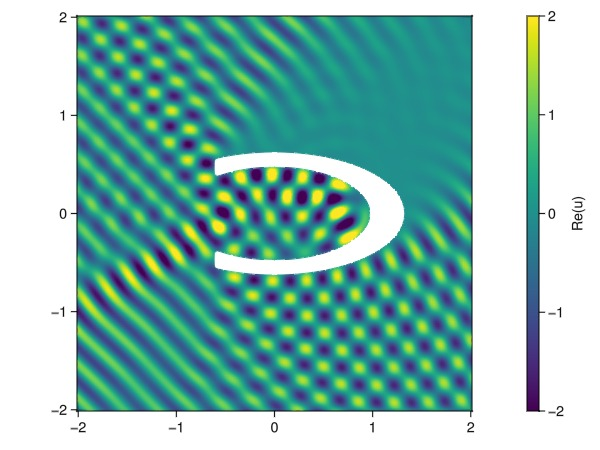
\includegraphics[width=0.6\linewidth]{images/cavity_fig.jpg}
    \caption{Geometry used in the test.}
    \label{fig:cavity_fig}
\end{figure}


Since the solution we search is the scattered field, $u$, produced by the incident wave $u_{i} = \exp^{ik(\vec{d}.\vec{x})}$, we still need to find the correct boundary condition in $\Gamma$ to obtain a unique solution.

Assuming the total field, $u_{t} = u_{i} + u $ satisfies a homogenous Neumann condition and that $u$ satisfies the Sommerfeld radiation condition, we have the following equations to the problem:

\begin{align}\label{eq:cavity_pdes}
    \begin{split}
        \Delta u + k^{2}u &= 0\\
        \partial_{n} u &= -\partial_{n}u_{i}\hspace{0.2in}, x \in \Gamma
    \end{split}
\end{align}

Which gives us, with \ref{eq:sol_bem}, all the mathematical formulation we need to continue with the applications.

Before going into each one of the results, we talk a little about both extremes of the performance evaluation in the inexact GMRES and matrix-vector problem. How to give an upper bound to the acceleration we expect?

If making the matrix-vector product's tolerance as 0 implies the use of the “original” matrix(remember using hierarchical matrices is already an approximation and therefore, not the original matrix), then we would expect 0$\%$ speedup.

A good way to infer the maximum acceleration possible for the inexact products would be using only admissible rank 1 blocks and measuring its execution time.

For doing that, we change the product tolerance to \textit{Infinity}, and the product will be realized with only rank-1 blocks, since it's programmed to get the first approximation lower than its given tolerance.

Of course, such thing would not happen in a practical situation, but it gives an upper bound for the speedup we should expect.

\section{Tolerance heuristic}

We mentioned the inexact product's tolerance multiple times throughout this study, but haven't really disclosed \textbf{how} to obtain it.
%FIXME: I forgot to add the article in the bibliography to cite them here...
As told in \autoref{chap:hmatrices}, the inexact matrix-vector product is adjusted with the number of columns used by each one of the subblocks during the operation. To convert one of the expressions in \autoref{eq:bound_E} or in \autoref{eq:boundE_final} to an integer, we use the following heuristic:

\begin{equation}
    n_{k} = \min \left(\frac{\epsilon}{\min(\tilde{r}_{k-1},1)},1 \right)
\end{equation}

Where $\tilde{r}_{k-1}$ is the residual of the previous iteration and $\epsilon$ the overall tolerance given to the inexact GMRES algorithm.

This expression is equivalent to take $\ell_{k} = 1$ in \autoref{eq:boundE_final}. Any of the other bounds showed in \autoref{chap:gmres} can be made by multiplying this expression by $\frac{\sigma_{k}(H_{k})}{k}$, $\frac{\sigma_{n}(A)}{k}$ or other values of $\ell_{k}$. A comparison between these different heuristics in the problem of a cavity scattering can be found below \ref{fig:bound_study}.

\section{Laplace's results}

%FIXME: put the correct values here
Setting our product tolerance to \textit{Infinity} and using only rank-1 blocks in the product, we got a () speedup.

All results are contained in \ref{fig:laplace_results}, showing the evolution of the residual with the product tolerance as well as the speedup to each of these values.

\begin{figure}[h!]
    \centering
    \includesvg[width=0.6\linewidth]{images/fixed_size_laplace_product.svg}
    \caption{Speedup and residual evolution for the product between a 8000x8000 HMatrix and a vector.}
    \label{fig:laplace_results}
\end{figure}

And since the matrix-product is accelerated, we should expect some speedup in the algorithm as well.

It should be noted that the acceleration is highly dependent on the compression of the coefficient matrix. Matrices with low maximum rank of each block would not receive a big boost, since the number of columns used for each subblock might not vary much with each different tolerance.

\section{Helmholtz's results}
%FIXME: Values here

\subsection{Matrix-vector product}

For a maximum speedup bound in the product, the infinity tolerance brought a () speedup.

For the unitary circle boundary the results can be seen in \ref{fig:Helmholtz_circle_results}, for both the matrix-vector product and an application of the Inexact GMRES with few iterations.

\begin{figure}[h!]
    \centering
    \begin{subfigure}[b]{0.45\linewidth}
        \includesvg[width=\linewidth]{images/fixed_size_helmholtz_product.svg}
        \caption{Results for the product of a 70000x 70000 HMatrix and a vector.}
    \end{subfigure}
    \begin{subfigure}[b]{0.45\linewidth}
        \includesvg[width=\linewidth]{images/fixed_size_helmholtz_gmres.svg}
        \caption{Results for an initial application of the Inexact GMRES algorithm.}
    \end{subfigure}
    \caption{Results for the application of the Inexact GMRES algorithm with a 70000x70000 HMatrix.}
    \label{fig:Helmholtz_circle_results}
\end{figure}

\subsection{Cavity scattering}

For the cavity, we start out by running smaller examples and study the bounds found of \autoref{chap:gmres}, mainly \ref{fig:bound_44} and \ref{eq:boundE_final}. Satisfying these bounds is a guarantee that the residual measured at each $k-th$ iteration, $\tilde{r_{k}}$, is close to the exact one $r_{k} = \norm{b-Ax_{k}}$.

%FIXME: Expliquer le setup numerique: qu est ce qu'on met la et qu est ce que ça veut dire
To verify the bounds found for $\norm{E_{k}}$, the perturbation of the coefficient matrix $A$ at each iteration, found in \ref{eq:bound_E} and \ref{eq:boundE_final}, We start with simple run in a smaller $A$ as to focus on the residues. We use $\sigma = 10^{-6}$ as the overall algorithm's tolerance for the solution, i.e., the iterations stop as soon as $\frac{b - Ax_{k}}{b} \leq sigma$ and the same $A$ that will be used later for a larger resolution cavity problem.

The plots are in \autoref{fig:bound_study}.

\begin{figure}[h!]
    \centering
    \begin{subfigure}[b]{0.45\linewidth}
        \includesvg[width=\linewidth]{images/bounds_44_normal.svg}
    \end{subfigure}
    \begin{subfigure}[b]{0.45\linewidth}
        \includesvg[width=\linewidth]{images/bounds_44_normal.svg}
    \end{subfigure}
    \caption{Multiple Images}
    \label{fig:multiple_figs}
\end{figure}


%FIXME: Mettre les deux figures une a cote de l autre
\begin{figure}[h!]
    \centering
    \includesvg[width=0.7\linewidth]{images/bound_study.svg}
    \caption{Evolution for each of the perturbation's bounds found in \autoref{chap:gmres}.}
    \label{fig:bound_study}
\end{figure}

This figure shows how the different bounds of the perturbation's behave through iterations. Recalling that a greater tolerance means a bigger room to work with larger perturbations of $A$, what can make the inexact matrix-vector product faster.


For the bounds in \ref{eq:borne_delta}, we have \autoref{fig:bound_44}.

\begin{figure}[h!]
    \centering
    \includesvg[width=0.7\linewidth]{images/bounds_44.svg}
    \caption{Evolution for each of the residual's bounds found in \autoref{chap:gmres}. Blue represents the difference between true and inexact residuals of the GMRES's solution and the other two, bounds this difference must satisfy.}
    \label{fig:bound_44}
\end{figure}

As we can look from both \autoref{fig:bound_study} and \autoref{fig:bound_44}, even if choosing $\ell_{k} = 1$ makes the inexact product's tolerance bigger, it still follows the restriction in the bound \ref{eq:borne_delta}. A test with these different choices for the product tolerance did not show a big variation between the iterations necessary for each one of them.

It could mean less strict tolerances can still lead to the algorithm's convergence, what can be used to accelerate the algorithm even further.

As for the speedup results, we have \autoref{fig:cavity_results}.

\begin{figure}[h!]
    \centering
    \includesvg[width=0.6\linewidth]{images/fixed_size_helmholtz_cavity.svg}
    \caption{Speedup witnessed in the application of the Inexact GMRES in a 50000×50000 matrix.}
    \label{fig:cavity_results}
\end{figure}

An evolution of the number of iterations in face of the different tolerances passed to the algorithm is in \ref{fig:cavity_iterations}.

\begin{figure}[h!]
    \centering
    \includesvg[width=0.6\linewidth]{images/fixed_size_helmholtz_cavity_iterations.svg}
    \caption{Evolution of the quantity of iterations needed for convergence and overall tolerance passed as an argument.}
    \label{fig:cavity_iterations}
\end{figure}



